% !TeX program = lualatex
% !TeX encoding = UTF-8
% グローバルチャレンジ2027 II 構築評価報告
% 必須: LuaLaTeX + LuaTeX-ja (TeX Live) / VS Code LaTeX Workshop
\documentclass[a4paper,10pt]{ltjsarticle}
\usepackage[top=19mm,bottom=20mm,left=18mm,right=18mm]{geometry}
\usepackage{graphicx}
\usepackage{hyperref}
\usepackage{xurl}
\usepackage{titlesec}
\usepackage{indentfirst} % 節・小節直後の段落も字下げする
\hypersetup{hidelinks,pdftitle={グローバルチャレンジ2027 IIにおける使用構築の事例分析と改善方針}}
\setlength{\columnsep}{8mm}
\setlength{\parindent}{\zw} % 段落冒頭は全角1文字分の字下げ
\setlength{\parskip}{0pt}
\renewcommand{\baselinestretch}{1.10}
\setlength{\textfloatsep}{9pt plus 2pt minus 2pt}
\setlength{\intextsep}{8pt plus 2pt minus 2pt}
\titleformat{\section}{\normalsize\bfseries}{\thesection.}{0.6em}{}
\titleformat{\subsection}{\normalsize\bfseries}{\thesubsection}{0.6em}{}
\titlespacing*{\section}{0pt}{1.5ex plus .4ex}{.6ex}
\titlespacing*{\subsection}{0pt}{1.1ex plus .3ex}{.4ex}
\pagestyle{plain}

% 編集箇所: 著者名や所属
\newcommand{\PaperAuthor}{ズズくん\qquad gurt}
\providecommand{\PaperAffiliation}{}

\begin{document}
\makeatletter
\twocolumn[
\begin{@twocolumnfalse}
  \begin{center}
    {\Large\bfseries 『Pokémon Champions』グローバルチャレンジ2027 IIにおける\\[1mm]
     使用構築の事例分析と改善方針\par}
    \vspace{1.6mm}
    {\normalsize ― トリックルーム展開と範囲攻撃の運用上の課題 ―\par}
    \vspace{3mm}
    {\normalsize\PaperAuthor\par}
    {\small\PaperAffiliation\par}
  \end{center}
  \vspace{2mm}
  \noindent\textbf{要旨（Abstract）}\par
  \small
  \noindent 本稿では、『Pokémon Champions』の公式オンライン大会「グローバルチャレンジ2027 II」における使用構築を対象に、18戦の対戦経験に基づいて運用上の課題と改善方針を検討する。メガフラエッテを中心とする構築に、リキキリンとコータスによるトリックルーム展開を組み込んだが、対戦終了時のレートは1500であった。対戦では、トリックルームの展開阻害、コータスの攻撃機会の不足、および味方への巻き込みによる範囲攻撃の使用制限が観察された。これらを踏まえ、行動順を確保する手段と、範囲攻撃を使用しやすい味方構成を改善候補として整理した。ただし、詳細な対戦記録を取得していないため、各課題が成績に及ぼした影響と、改善案の有効性は未検証である。\par
  \vspace{1.5mm}
  \noindent\textbf{キーワード：}Pokémon Champions、ダブルバトル、レギュレーションM-C、トリックルーム、リキキリン・コータス、範囲攻撃\par
  \vspace{3mm}\hrule\vspace{3mm}
\end{@twocolumnfalse}
]
\makeatother
\normalsize

\suppressfloats[t] % 最初の左段には上部の図を置かず、右段へ送る。
\section{はじめに}
\subsection{背景}

本大会「グローバルチャレンジ2027 II」は、ポケモンジャパンチャンピオンシップス2027 マスターカテゴリ（以下、PJCS2027）の予選出場権獲得に向けた公式オンライン大会である。全6回のグローバルチャレンジの第2回に該当し、レギュレーションM-Cのダブルバトルによって実施された。各カテゴリの上位入賞者にはPJCS2027予選への出場権が付与される\cite{pjcs}。

% 図を左段の早い位置で宣言し、右段上部への配置を促す。
\begin{figure}[t]
  \centering
  \IfFileExists{figures/party.png}{%
    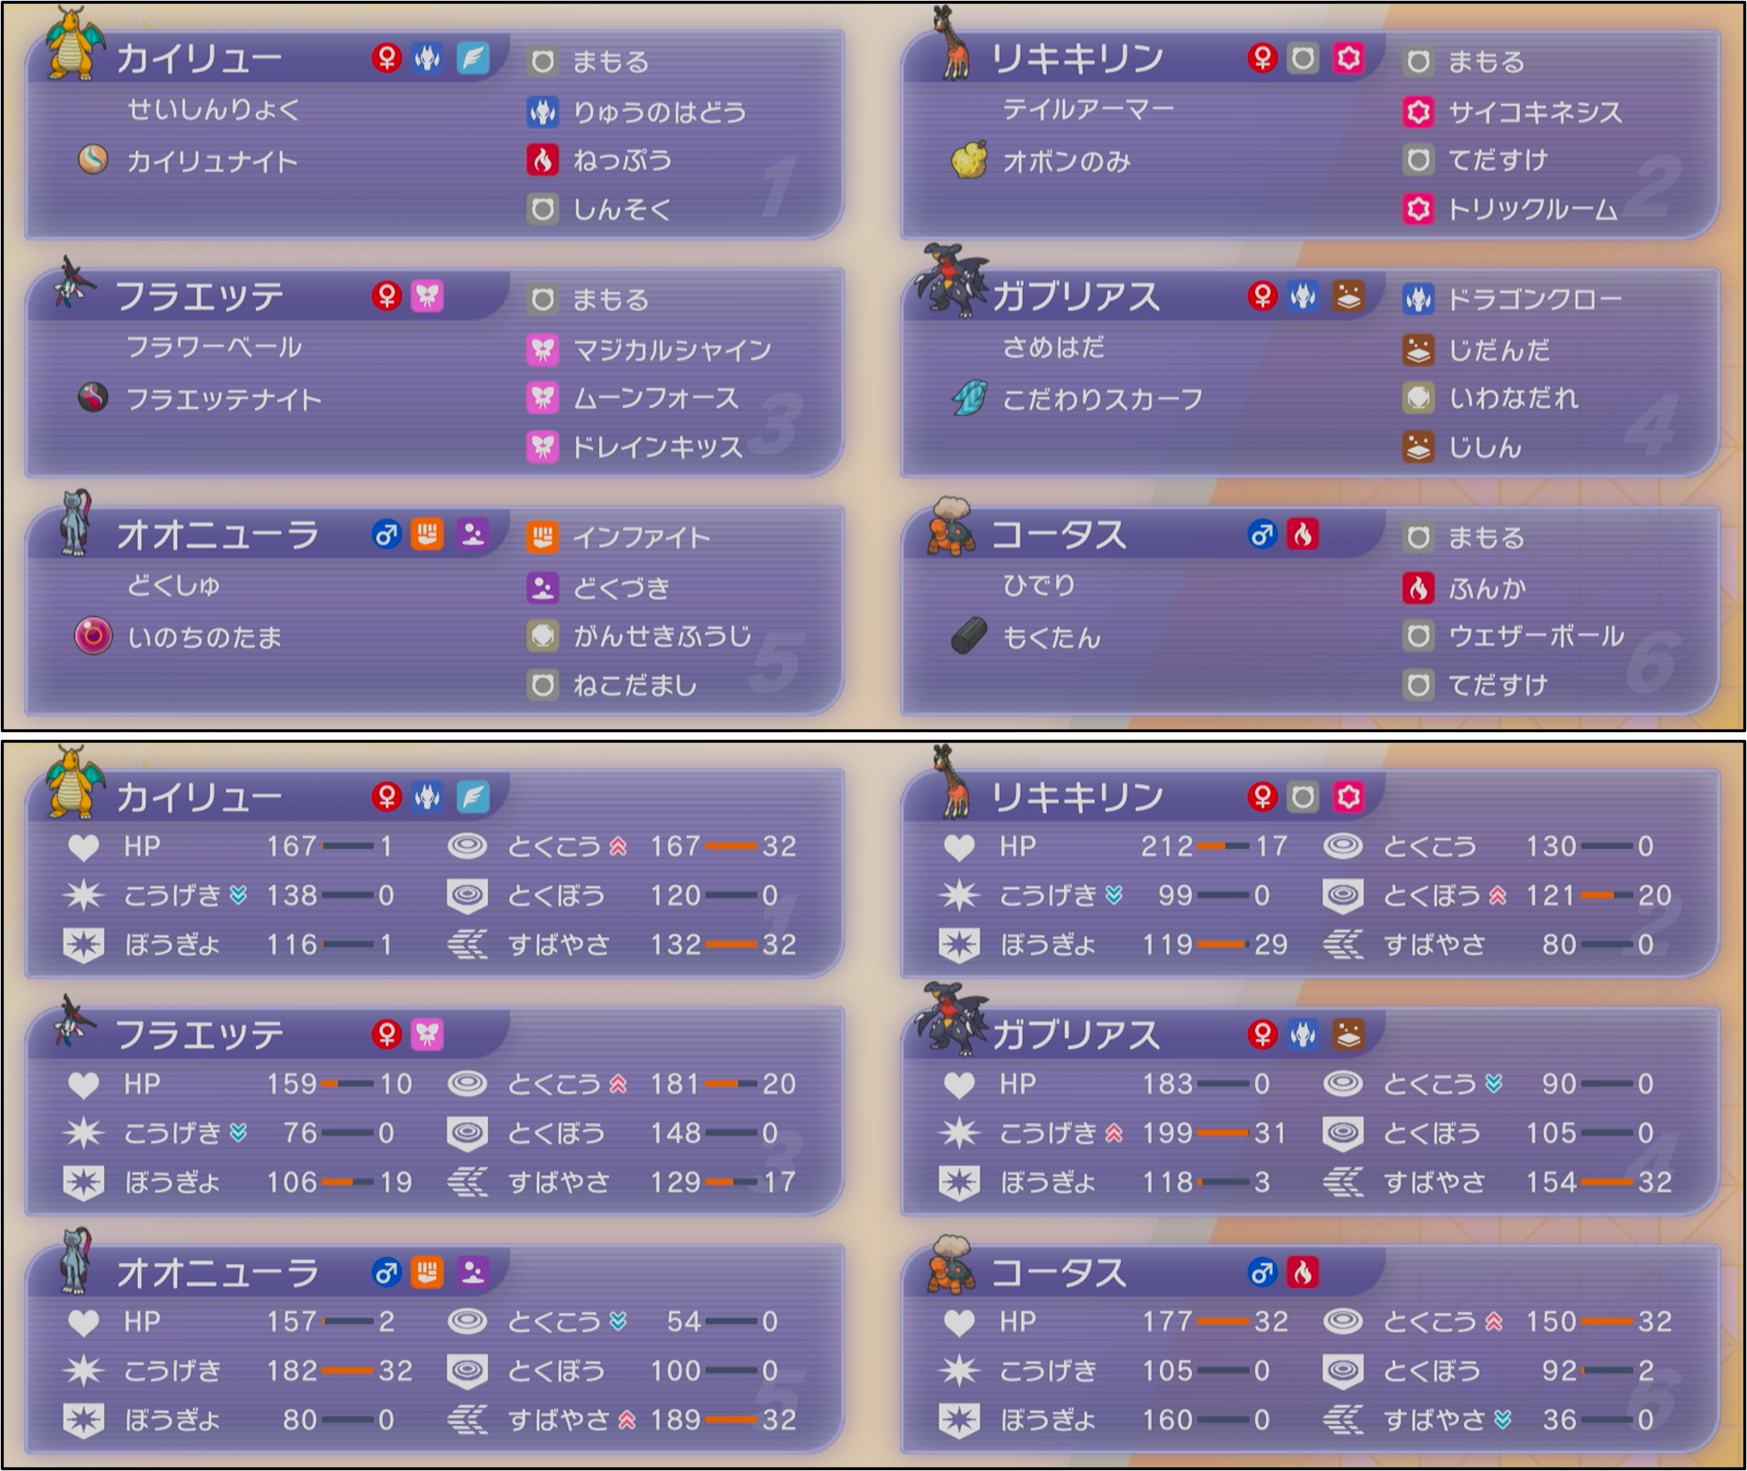
\includegraphics[width=\linewidth]{figures/party.png}%
  }{%
    \fbox{\begin{minipage}[c][37mm][c]{0.92\linewidth}
      \centering\small [ここにパーティ構成の画像]\\[2mm]
      \footnotesize \texttt{figures/party.png} に画像を置くと自動挿入
    \end{minipage}}%
  }
  \caption{グローバルチャレンジ2027 IIで使用した構築}
  \label{fig:party}
\end{figure}

本大会では、幅広い相手に対応できるパーティを目指し、構築選択において汎用性と安定性を重視した。対戦の運用はズズくんが実施した。対戦者は予選出場権の獲得を目指してレート1700台半ばを目標に設定したが、この数値は対戦者の見通しに基づくものであり、公式な出場権付与の基準ではない。

前回の「グローバルチャレンジ2027 I」では、メガボーマンダを中心とした構築を使用し、約1660のレートを記録した。今回は目標への到達を目指し、以前のレギュレーションM-Bで使用経験のある構築を基礎として、操作への習熟を活かす方針を採った。

\subsection{目的}

本稿の目的は、18戦の対戦経験から使用構築の運用上の課題を整理し、今後検証する改善案を示すことである。各ポケモンの役割遂行、味方との相性補完、および相手の行動予測への依存度という観点から分析する。

前回大会やレギュレーションM-Bでの運用経験も、課題を検討するための参考とする。ただし、これらは条件を統一した比較ではない。本稿は今回の対戦を対象とした事例分析であり、構築性能の優劣や成績差の原因を確定するものではない。

\section{使用構築と評価方法}
\subsection{構築方針}

本大会では、特定の技の成立だけに勝ち筋を依存させず、相手に応じて攻撃、補助技、交代を選択するスタンダード構築を基本方針とした。中心にはメガフラエッテを採用し、補助的な勝ち筋としてリキキリンとコータスによるトリックルーム展開を組み込んだ。

リキキリンには「トリックルーム」と「てだすけ」による支援、コータスには特性「ひでり」で形成する晴れ状態での「ふんか」による範囲攻撃を想定した。「ふんか」はHP残量が多いほど威力が高いため、コータスが被弾する前に攻撃できる状況を形成することが、この戦術の前提となる。

対戦者はレギュレーションM-Bでこの組み合わせを運用した経験があり、役割と基本的な行動選択を把握していた。既存の運用経験を活かし、対戦中の判断負担を抑えることも採用理由とした。

\subsection{使用パーティ}

本構築は、メガフラエッテ、メガカイリュー、リキキリン、ガブリアス、オオニューラ、コータスの6匹で構成される（図\ref{fig:party}）。メガフラエッテとメガカイリューを相手に応じて選択するメガシンカ候補として採用し、リキキリンとコータスのトリックルーム展開を補助的な勝ち筋とした。また、ガブリアスの攻撃性能と技範囲、オオニューラの「ねこだまし」による行動制限を組み合わせ、トリックルームに依存しない立ち回りも可能になることを想定した。

\subsection{評価対象と分析手順}

大会の開催期間は2026年10月30日から11月2日であり、対戦ルールはレギュレーションM-Cのダブルバトルである\cite{pjcs}。評価対象は、対戦者が本大会で実施した18戦とする。

分析には、対戦終了時のレートと、対戦者自身による対戦中の観察の振り返りを用いた。想定した役割と実際に選択できた行動を照合し、攻撃や支援を実行できなかった場面を整理した。そのうえで、行動順、味方との相性、および相手の行動予測との関係から説明を検討し、改善案を導いた。勝敗数、選出回数、技の使用回数などの詳細な記録は取得していないため、以下の結果は定性的な観察として扱う。

本稿では、汎用性を異なる相手の構成や行動に対して有効な選択肢を確保できること、安定性を想定した攻撃や支援を実行しやすいことと定義する。また、頑健性は、相手の行動予測が外れた場合にも攻撃機会や勝ち筋を維持できることを指す。これらは分析の観点であり、本稿では数値化して比較していない。

\section{結果}
\subsection{大会成績}

本大会では計18戦を実施し、対戦終了時のレートは初期値と同じ1500であった。勝敗数を記録していないため、勝率は算出できない。

最終レートは前回大会の約1660を約160下回り、目標とした1700台半ばにも到達しなかった。ただし、両大会で使用構築、対戦相手、対戦数が異なるため、この差だけでは構築性能の優劣を判断できない。

\subsection{トリックルーム展開の運用結果}

リキキリンが相手の攻撃によって「トリックルーム」を使用する前に倒される場面や、「ふういん」によって使用を阻害される場面が観察された。

トリックルーム成立後にも、雨状態への天候変更や、ほのおタイプの攻撃に耐性を持つ相手との対面によって、コータスの「ふんか」で相手を倒しきれない場面があった。コータスが天候を変更したものの、想定した攻撃役としての役割を果たせない場面も観察された。その際、リキキリンによる「てだすけ」を組み合わせても相手を倒すには至らなかった。

\subsection{メガフラエッテの運用結果}

対戦者は、メガフラエッテについて、相手に応じて攻撃技を選択しやすく、構築の中心として運用できたと評価した。「ドレインキッス」で攻撃しながらHPを回復し、場に残って再度攻撃する場面が観察された。一方、従来採用していた「はめつのひかり」を外したことで、その一撃による突破を狙う選択肢は失われた。

\subsection{メガカイリューの運用結果}

メガカイリューは、HP満タン時に特性「マルチスケイル」で被ダメージを抑え、初手の攻撃を耐えて行動する場面があった。一方、一度の攻撃で相手を倒しきれず、追加の攻撃機会を必要とする場面も観察された。

「ねっぷう」は相手2体を攻撃する手段として使用したが、技が命中せず、反撃によって倒される場面があった。特にはがねタイプやこおりタイプの相手に対して、攻撃を命中させられない場合の反撃が問題となった。

\subsection{ガブリアスの運用結果}

ガブリアスは、「じだんだ」「ドラゴンクロー」「いわなだれ」「じしん」によって相手に応じた攻撃を選択できた。「いわなだれ」では相手2体にダメージを与え、追加効果の「ひるみ」によって相手の行動を阻害する場面もあった。

一方、「じしん」は味方への巻き込みによって使用を制限された。今回の構築では、味方のうちじめんタイプの攻撃を無効化できるポケモンがカイリューに限られ、それ以外の味方と並ぶ場面では別の技を選択する必要があった。

\subsection{オオニューラの運用結果}

オオニューラでは、相手の特性「いかく」で攻撃を下げられ、「いのちのたま」を持っていても相手を倒しきれず、反撃によって倒される場面があった。また、サイコフィールドと「ワイドフォース」を組み合わせた相手に対して、行動する前に倒される場面が観察された。

\subsection{構築全体の攻撃機会}

コータスの「ふんか」は展開阻害や天候変更によって、ガブリアスの「じしん」は味方への巻き込みによって使用を制限された。メガフラエッテの「マジカルシャイン」は使用しやすかった一方、相手を倒すために単体攻撃を選択する場面もあった。相手の「まもる」や交代の予測が外れ、狙った相手を倒せず不利になる場面が観察された。

\section{考察}
\subsection{トリックルーム展開と攻撃機会の関係}

観察された展開阻害とコータスの攻撃機会の不足は、トリックルームを成立させるまでの負担と、成立後に得られる利益との不均衡によって説明できる可能性がある。

「トリックルーム」の通常の優先度は$-7$であり、一般的な攻撃技より後に使用する。このため、展開役は発動前に相手の攻撃や妨害を受けやすい。コータスは素早さが低いうえ、「ふんか」の威力がHP残量に依存するため、トリックルームが成立しなければ先に被弾して攻撃性能を損なう可能性がある。一方、成立させても天候変更や相手の耐性によって十分なダメージを与えられない場合、展開に費やした行動を攻撃成果につなげにくい。

また、コータスが相手を倒せない場合、「てだすけ」によるリキキリンの支援も成果につながりにくい。このように、支援役と攻撃役の役割が相互に依存していたことが、今回の構築における不安定さの一因と考えられる。ただし、この観察から両者の組み合わせ自体の有効性を否定することはできない。選出や行動選択、遭遇した相手との相性も別の説明となり得る。

レギュレーションM-Bでの運用時には、この組み合わせが有効だったという対戦者の評価がある。しかし、当時との成立率や相手の構成を比較できる記録はないため、今回の課題を環境全体の変化に帰することはできない。

\subsection{「おいかぜ」の展開速度と効果の適用範囲}
\label{sec:tailwind}

「トリックルーム」と「おいかぜ」の比較では、発動までに受ける妨害と、発動したターンに得られる攻撃機会を区別する必要がある。トリックルームは通常の攻撃より後に発動するため、展開役が被弾してから行動することになる。発動前の被弾は、ひんしに加え、「いわなだれ」のひるみなどの追加効果によって、発動そのものを阻害される機会にもなる。

一方、「おいかぜ」の通常の優先度は$0$であり、同じ優先度の相手より使用者の素早さが高ければ、相手の攻撃を受ける前に使用できる。また、特性「いたずらごころ」によって優先度が$+1$となる場合、通常の優先度$0$の攻撃に先んじて展開できる。このため、トリックルームと比較して、展開前の被弾やひるみによる中断を回避できる場面がある。

おいかぜの効果は発動したターンの行動順にも反映される。まだ行動していない味方が、素早さの上昇によって同じ優先度の相手を上回れば、そのターンから先に攻撃できる。高火力の技で相手を倒すことができれば、相手の攻撃や妨害が実行される前に行動を阻止できる。通常は相手の攻撃後に発動するトリックルームに対し、おいかぜには展開と攻撃を同じターンに結び付けやすい利点がある。

効果の適用範囲も異なる。トリックルームは両陣営の行動順に作用するため、相手の低速なポケモンにも先に行動する機会を与え得る。一方、おいかぜが素早さを2倍にするのは使用者側だけであり、相手を直接強化せずに行動順の改善を図れる\cite{speedcontrol}。したがって、相手の低速なポケモンによる効果の利用を考慮する負担を抑えやすい。

以上の特徴は、今回観察された展開前の行動阻害と、攻撃機会の不足に対応する理由となる。相手より先においかぜを使用できる展開役と、効果中に相手を上回る素早さと攻撃性能を持つ味方を組み合わせるならば、今回遭遇した相手への対応では、トリックルームよりもおいかぜの方が適していると考えられる。ただし、コータスのような低速の攻撃役をそのまま使用しても、素早さ2倍だけで先に動けるとは限らないため、攻撃役を含めた構築の変更が前提となる。

おいかぜも、優先度の高い「ねこだまし」や、先に使用された「ちょうはつ」などによって阻害される。また、相手のおいかぜによって素早さの差を解消されたり、トリックルームによって素早さの上昇が不利に働いたりする場合がある。したがって、ここでの比較は今回の課題に対する改善仮説であり、環境全体での優位性の実証とは区別する。

\subsection{行動順と範囲攻撃による予測への依存度の低減}

相手より先に攻撃して倒したり、追加効果で行動を阻害したりできれば、相手が予定した行動を実行する前に有利な状況を形成できる。このため、攻撃性能だけでなく、攻撃機会を確保するための行動順も構築の評価対象となる。

範囲攻撃は相手2体を同時に攻撃できるため、単体攻撃と比較して攻撃対象の予測への依存度を低減できる可能性がある。ただし、「まもる」、交代、無効化や防御の手段によって成果は変わる。範囲攻撃であれば常に有利になるわけではなく、実際に使用できる条件と、相手を倒すために必要なダメージを併せて検討する必要がある。

前回大会では、サーフゴーの「ゴールドラッシュ」と、素早さの高いポケモンによる攻撃が有効だったとの評価がある。この経験は、行動順と範囲攻撃を組み合わせる改善案の参考となるが、今回の構築との性能差を実証するものではない。

\subsection{想定した対戦傾向と実際の行動選択の不一致}

対戦者は、ランクマッチで経験した行動傾向を参考に相手の行動を予測していた。しかし、本大会では想定と異なる行動を取られ、狙った相手を倒せない場面があった。このため、特定の行動傾向を前提とした立ち回りが、今回遭遇した相手に適合しなかった可能性がある。

ただし、相手のレート帯と行動傾向の関係を示す記録はなく、予測の不一致をレート帯の違いによって説明することはできない。対戦者の予測そのものや、行動候補の見落としにも検討の余地がある。

改善にあたっては、特定の行動を予測した場合の利益だけでなく、予測が外れた場合にも攻撃機会を残せるかを評価する必要がある。複数の行動候補に対して有効となり得る範囲攻撃や、相手より先に攻撃できる手段は、そのための候補となる。

\subsection{メガフラエッテの継戦能力とメガカイリューの反撃への耐性}
\label{sec:mega-comparison}

メガフラエッテの「ドレインキッス」は、攻撃しながらHPを回復できる点で継戦能力に寄与すると考えられる。一方、「はめつのひかり」による一度の攻撃での突破とは役割が異なる。今回の観察だけでは優劣を決められないため、回復によって得られる追加の攻撃機会と、一撃で相手を倒す必要がある場面を比較することが課題となる。

メガカイリューの「ねっぷう」の評価では、攻撃が命中しない可能性に加え、その後の反撃を耐えられるかが重要となる。特に、はがねタイプやこおりタイプの相手からの反撃を耐えるために「マルチスケイル」が必要となる場面では、HP満タンの維持が攻撃機会の確保に関わる。事前の被弾によって特性の効果を失うと、「ねっぷう」が命中しなかった後に場へ残ることが難しくなる。

比較候補のメガリザードンYは、メガカイリューより特攻が高く、自身の特性「ひでり」で晴れ状態を形成できる。このため、天候変更と晴れ状態での「ねっぷう」による攻撃を1匹で担える点に利点がある。

防御面では、メガリザードンYは、はがねタイプやこおりタイプの相手からの反撃に対して、自身のタイプ相性を活かして耐えられる場面がある。メガカイリューでは「マルチスケイル」の維持が必要となる場面でも、メガリザードンYは同特性による被ダメージ軽減を必要とせず、反撃後に再度攻撃できる可能性がある。したがって、両者の比較では、攻撃性能に加え、HP満タンの維持にどの程度依存して行動回数を確保するかという違いが重要となる。

\subsection{味方との相性補完と攻撃回数の確保}

ガブリアスの「じしん」の使用制限は、技の性能だけでなく、味方との組み合わせが攻撃機会を左右することを示す事例である。じめんタイプの攻撃を無効化できる味方の確保に加え、味方の「まもる」などを含む行動の組み合わせも検討対象となる。

オオニューラについては、一度の攻撃を強化しても相手を倒せない場合、反撃と「いのちのたま」によるHP消費が次の攻撃機会を制限し得る。このため、持ち物を変更して行動回数を増やすことが改善候補となる。ただし、持ち物による威力補正を失う影響もあるため、総ダメージ量や勝率が向上するかは別途検証する必要がある。

\section{今後の構築改善方針}
\subsection{改善候補と検証項目}

今回の観察から導いた改善候補を表\ref{tab:improvements}に示す。いずれも効果を実証したものではない。行動順を確保する手段と、範囲攻撃を使用できる味方構成を優先的に検討し、複数の変更を同時に行う場合は、個別の効果を切り分けられないことに留意する。

\begin{table}[t]
  \centering
  \caption{運用上の課題に対する改善候補と検証項目}
  \label{tab:improvements}
  \footnotesize
  \setlength{\tabcolsep}{3pt}
  \renewcommand{\arraystretch}{1.18}
  \begin{tabular}{@{}p{0.22\linewidth}p{0.33\linewidth}p{0.36\linewidth}@{}}
    \hline
    課題 & 改善候補 & 検証項目 \\
    \hline
    展開前の被弾・妨害 & トリックルームへの依存を抑え、「おいかぜ」を検討 & 展開の成立、発動ターンの味方の行動順と攻撃成果 \\
    範囲攻撃の使用制限 & 高火力の範囲攻撃と、味方への巻き込みを抑える構成 & 使用機会、命中の成否、与ダメージ、味方への損失 \\
    「いわなだれ」による行動阻害 & 「ワイドガード」やブリジュラスの採用 & 被ダメージと、ひるみによる行動阻害の有無 \\
    天候変更役と攻撃役の分離 & メガリザードンYによる役割の統合 & 天候変更後の攻撃機会、メガシンカ候補の選択 \\
    オオニューラの行動回数不足 & 「きあいのタスキ」や各種シードの採用 & 攻撃回数、総ダメージ量、相手を倒せたか \\
    回復と一撃での突破の両立 & 「ドレインキッス」と「はめつのひかり」の比較 & 回復後の追加行動、一撃で倒す必要がある場面 \\
    \hline
  \end{tabular}
\end{table}

「おいかぜ」は、\ref{sec:tailwind}節で述べた発動ターンからの攻撃機会を活かすため、展開役が相手より先に使用できるかと、効果を受けた味方が相手より先に攻撃できるかを併せて評価する。素早さの設定と展開役への妨害対策を具体化し、発動したターンに攻撃できたか、その攻撃によって相手の行動を阻止できたかを確認する。

「いわなだれ」への対策では、被ダメージの軽減と、ひるみによる行動阻害への対応を区別する。「ワイドガード」は技そのものへの防御手段となる一方、ブリジュラスの耐性や特性「じきゅうりょく」は、被弾後の継戦に寄与しても、ひるみ自体を防ぐものではない。相手が同じ技を繰り返すことへの抑止効果と、こちらが実際に行動できたかを分けて記録する。

オオニューラの持ち物については、「きあいのタスキ」によってHP満タン時の一撃によるひんしを防ぐ案と、対応するフィールドでシードを使用する案を検討する。後者ではフィールドを形成する手段が必要であり、持ち物単独ではなく構築全体の変更として評価する。

\subsection{メガリザードンYによる役割の統合}

メガリザードンYは、\ref{sec:mega-comparison}節で述べた攻撃面と防御面の特徴に加え、コータスの天候変更とメガカイリューの範囲攻撃を1匹に集約する候補となる。メガシンカ時に「ひでり」が発動するため、交代による天候変更が先に処理される状況では、相手の交代で雨状態となった後に晴れへ変更することも狙える。

一方、メガフラエッテとのメガシンカ枠の競合が生じる。同じ対戦で両者をメガシンカさせることはできないため、コータスで晴れを形成してからメガフラエッテで攻撃する従来の組み合わせを、そのまま置き換えることはできない。天候変更と攻撃の役割を統合する利点に加え、相手に応じてどちらをメガシンカさせるか、残りの味方でどの役割を補うかを検討する必要がある。

\subsection{改善効果の検証方法}

今後は、対戦ごとに使用構築、勝敗、対戦前後のレート、選出、主要な技の使用と成否を記録する。トリックルームや「おいかぜ」については、使用を試みた回数、成立した回数、および成立後の攻撃機会を記録する。特においかぜでは、発動したターンの味方の行動順と、相手の行動を阻止できたかを確認する。範囲攻撃については、実際の使用回数に加え、味方への巻き込みや相手の防御手段によって使用を見送った場面も整理する。

敗戦時には、最後に倒された場面だけでなく、展開の阻害、命中しなかった攻撃、攻撃対象の予測など、結果に関わったと考えられる事象を記録する。変更前後で可能な限りルールと対戦条件をそろえ、勝率だけでなく、各改善案が対象とする行動機会の変化を確認する。

\section{本分析の限界}

評価対象は単一の対戦者による18戦であり、詳細な対戦記録を取得していない。観察には印象的な場面を重視する偏りや振り返りの誤差が含まれ得るため、各事象の頻度や成績への寄与を定量的に評価することはできない。

対戦者の認識では相手は主にレート1500付近であったが、相手ごとのレートや構成を集計していない。したがって、遭遇した戦術が大会全体を代表するとはいえず、雨構築や特定の耐性を持つポケモンの増減、レート帯ごとの行動傾向を論じることはできない。

前回大会とのレート差や、レギュレーションM-Bでの運用経験との違いも、構築変更だけでは説明できない。前回大会は今回と同じレギュレーションM-Cであったが、使用構築、対戦相手、対戦数が異なる。対戦者の行動選択や、技の命中などの偶然性も結果に関わり得る。

また、メガリザードンYなどの改善候補は、今回の18戦で比較評価したものではない。本稿で示した運用上の課題と改善案は、今後の記録と検証に向けた仮説として位置付けられる。

\section{結論}

本稿では、グローバルチャレンジ2027 IIにおける18戦の対戦経験から、使用構築の運用上の課題を整理した。対戦終了時のレートは1500であり、対戦ではトリックルームの展開阻害、コータスの攻撃機会の不足、および味方への巻き込みによる範囲攻撃の使用制限が観察された。

これらを踏まえ、行動順を確保する手段、範囲攻撃を使用しやすい味方構成、および反撃後にも攻撃機会を残す運用を改善候補として示した。ただし、各課題が成績に及ぼした影響と改善案の有効性は未検証である。今後は詳細な対戦記録を蓄積し、想定した行動を実行できたかと、予測が外れた場合に攻撃機会を維持できたかを確認する。

\begin{thebibliography}{9}
\bibitem{pjcs} 株式会社ポケモン，「『Pokémon Champions』チャンピオンシップシリーズ『2027シーズン』について」，『Pokémon Champions』公式お知らせ（オンライン）．\url{https://champions-news.pokemon-home.com/ja/page/833.html}（参照2026年11月2日）．
\bibitem{speedcontrol} Chris Han, ``Get Ready for Regionals with Pokémon VGC Expert Chris Han,'' Pokemon.com（オンライン）．\url{https://www.pokemon.com/us/features/get-ready-for-regionals-with-pokemon-vgc-expert-chris-han}（参照2026年11月2日）．
\end{thebibliography}
\end{document}
